\documentclass[12pt,a4paper]{article}
\usepackage[utf8]{inputenc}
\usepackage[T1]{fontenc}
\usepackage{amsmath, amssymb, amsfonts}
\usepackage{mathrsfs}
\usepackage{hyperref}
\usepackage{geometry}
\usepackage{graphicx}
\geometry{margin=2.5cm}

\title{\bfseries Transformée de Laplace inverse de \(\displaystyle G(s)=\frac{\ln|s|}{\sqrt{1+s^2}}\)}
\author{Nom: RANDRIAMANANTENA \\
Prénoms: Tsiky Ny Antsa \\
Matricule: 00550-80-23 \\
Parcours: Génie Logiciel}
\date{}

\begin{document}
\maketitle

\section{Introduction}
On s'intéresse à la fonction
\[
G(s) = \frac{\ln|s|}{\sqrt{1+s^2}}, \qquad \Re(s)>0,
\]
où l'on interprète la valeur absolue comme la détermination principale du logarithme pour \(s\) complexe.
Dans la suite on se placera dans le cas réel \(s>0\) pour simplifier, ce qui donne
\[
G(s) = \frac{\ln s}{\sqrt{1+s^2}}, \qquad s>0.
\]
On cherche la fonction causale \(g(t)\) telle que
\[
\mathcal{L}\{g(t)\} = \int_{0}^{\infty} g(t)\,e^{-st}\,dt = G(s).
\]

La réponse fait intervenir la fonction de Bessel \(J_0\) et la fonction digamma \(\psi\) (dérivée logarithmique de la fonction Gamma). Nous allons détailler les étapes qui mènent à l'expression explicite de \(g(t)\).

\section{Outils nécessaires}
\subsection{Fonction de Bessel \(J_0\)}
La fonction de Bessel d'ordre zéro admet le développement en série entière
\begin{equation}\label{eq:J0series}
J_0(t) = \sum_{n=0}^{\infty} \frac{(-1)^n}{4^n\,(n!)^2}\, t^{2n},
\end{equation}
et sa transformée de Laplace est bien connue :
\begin{equation}\label{eq:LJ0}
\mathcal{L}\{J_0(t)\} = \frac{1}{\sqrt{1+s^2}}, \qquad \Re(s)>0.
\end{equation}

\subsection{Fonction digamma \(\psi\)}
La fonction digamma est définie par
\[
\psi(z) = \frac{d}{dz}\ln\Gamma(z) = \frac{\Gamma'(z)}{\Gamma(z)}.
\]
Elle satisfait la propriété \(\psi(1)=-\gamma\) (constante d'Euler-Mascheroni) et la formule de récurrence \(\psi(z+1)=\psi(z)+\frac{1}{z}\).
Nous utiliserons le résultat suivant (obtenu par dérivation sous le signe intégral de la transformée de Laplace de \(t^{\nu}\)) :
\begin{equation}\label{eq:inverseLog}
\mathcal{L}^{-1}\!\left\{ \frac{\ln s}{s^{\nu+1}} \right\}
= \frac{t^{\nu}}{\Gamma(\nu+1)}\bigl(\psi(\nu+1) - \ln t\bigr),
\quad \Re(\nu)>-1,\; \Re(s)>0.
\end{equation}

\section{Inversion par développement en série}
Pour inverser \(G(s) = \ln s \cdot (1+s^2)^{-1/2}\), nous développons d'abord \((1+s^2)^{-1/2}\) en série de puissances de \(s^{-1}\) (valable pour \(|s|>1\)) :
\[
\frac{1}{\sqrt{1+s^2}}
= \frac{1}{s}\left(1+\frac{1}{s^2}\right)^{-1/2}
= \sum_{n=0}^{\infty} \binom{-\frac12}{n} s^{-2n-1}
= \sum_{n=0}^{\infty} \frac{(-1)^n (2n)!}{4^n\,(n!)^2}\, s^{-2n-1}.
\]
Ainsi,
\[
G(s) = \ln s \sum_{n=0}^{\infty} \frac{(-1)^n (2n)!}{4^n\,(n!)^2}\, s^{-2n-1}
= \sum_{n=0}^{\infty} \frac{(-1)^n (2n)!}{4^n\,(n!)^2}\,
\frac{\ln s}{s^{2n+1}}.
\]

Appliquons maintenant \eqref{eq:inverseLog} avec \(\nu = 2n\). On a \(\Gamma(2n+1) = (2n)!\), donc
\[
\mathcal{L}^{-1}\!\left\{ \frac{\ln s}{s^{2n+1}} \right\}
= \frac{t^{2n}}{(2n)!}\bigl(\psi(2n+1) - \ln t\bigr).
\]

Par linéarité de la transformée inverse, on obtient
\begin{align}
g(t) &= \sum_{n=0}^{\infty} \frac{(-1)^n (2n)!}{4^n\,(n!)^2}\,
\frac{t^{2n}}{(2n)!}\bigl(\psi(2n+1) - \ln t\bigr) \notag\\
&= \sum_{n=0}^{\infty} \frac{(-1)^n}{4^n\,(n!)^2}\, t^{2n}\,
\bigl(\psi(2n+1) - \ln t\bigr). \label{eq:series}
\end{align}

\section{Identification des fonctions de Bessel}
La somme dans \eqref{eq:series} se décompose en deux parties :
\[
g(t) = - \ln t \sum_{n=0}^{\infty} \frac{(-1)^n}{4^n\,(n!)^2}\, t^{2n}
\;+\; \sum_{n=0}^{\infty} \frac{(-1)^n}{4^n\,(n!)^2}\, t^{2n}\,\psi(2n+1).
\]
D'après \eqref{eq:J0series}, la première somme est exactement \(J_0(t)\).
Par conséquent,
\[
\boxed{%
g(t) = -\,J_0(t)\,\ln t \;+\; \sum_{n=0}^{\infty} \frac{(-1)^n}{4^n\,(n!)^2}\,
t^{2n}\,\psi(2n+1)
}. \label{eq:final}
\]

C'est la transformée de Laplace inverse cherchée.

\section{Propriétés de la solution}
\begin{itemize}
\item \textbf{Comportement près de l'origine} (\(t\to 0^{+}\)) : \\
\(J_0(0)=1\) et seul le terme \(n=0\) de la série contribue, avec \(\psi(1)=-\gamma\). Donc
\[
g(t) \sim -\ln t - \gamma \quad (t\to 0^{+}),
\]
ce qui tend vers \(+\infty\).

\item \textbf{Convergence de la série} : Le rayon de convergence de la série entière est infini (grâce au facteur \((n!)^{-2}\)), donc \(g(t)\) est définie pour tout \(t\geq 0\). La série converge rapidement pour des arguments modérés ; pour \(t\) grand, des approximations asymptotiques peuvent être préférées.

\item \textbf{Oscillations} : La présence de \(J_0(t)\), fonction oscillante amortie, confère à \(g(t)\) un comportement oscillatoire avec une amplitude décroissant comme \(t^{-1/2}\) lorsque \(t\to\infty\).

\item \textbf{Représentation intégrale} : En utilisant le produit de convolution et la relation \(\mathcal{L}\{\ln t\} = -\frac{\gamma+\ln s}{s}\), on peut aussi exprimer \(g(t)\) sous la forme
\[
g(t) = -\frac{d}{dt}\left[\int_{0}^{t} \ln(u)\,J_0(t-u)\,du\right] - \gamma\,J_0(t).
\]
\end{itemize}

\section{Conclusion}
Nous avons établi l'expression exacte de la transformée de Laplace inverse de \(G(s)=\ln|s|/\sqrt{1+s^2}\) en faisant intervenir la fonction de Bessel \(J_0\) et la fonction digamma \(\psi\). La démarche repose classiquement sur le développement en série du facteur \((1+s^2)^{-1/2}\) et l'inversion terme à terme de \(\ln s / s^{\nu+1}\). La solution obtenue est
\[
g(t) = -J_0(t)\ln t + \sum_{n=0}^{\infty} \frac{(-1)^n}{4^n\,(n!)^2}\, t^{2n}\,\psi(2n+1),
\]
valable pour \(t>0\).

\begin{figure}[h!]
\centering
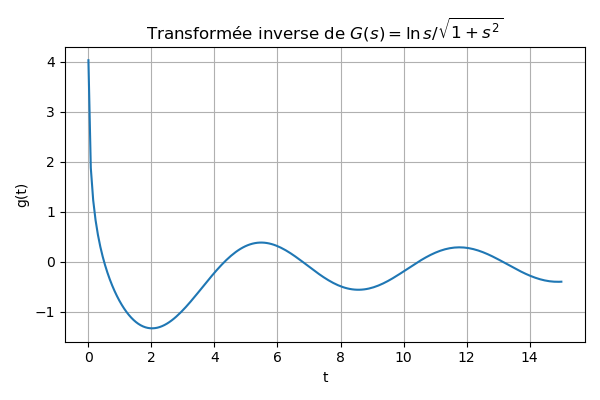
\includegraphics[width=0.95\textwidth]{g_t.png}
\caption{Tracé de la fonction $g(t)$ généré par le code de vérification.}
\label{fig:g_t}
\end{figure}

\vspace{1cm}
\begin{center}
\rule{0.5\textwidth}{0.4pt}
\end{center}
\textit{Références :} \\
Tables de transformées de Laplace, fonctions spéciales (Bessel, Gamma, digamma), propriétés des séries entières.

\end{document} 
